\documentclass[nofilelist,dvipsnames]{cslthse-msc}
% to show a list of used packages at the end of the document, delete the nofilelist option
%\documentclass{cslthse-msc}
%\setlength{\textfloatsep}{1pt plus 1.0pt minus 2.0pt}
\usepackage[utf8]{inputenc}
\usepackage[english]{babel}
\usepackage{amsmath}
\usepackage{amsthm}
\usepackage{graphicx}
\usepackage[titletoc, header, page]{appendix}
\usepackage{transparent}
\usepackage[
	backend=biber,
	style=numeric,
	sorting=none,
]{biblatex}
\addbibresource{report.bib}
%\setlength{\belowcaptionskip}{0pt}
\usepackage{parskip}
\usepackage{textcomp}
\usepackage{pdfpages}

% used to display the used files at the end. Select nofilelist as a package option to disable this
%\listfiles % initialize

%\geometry{showframe}
%better like this?
%\student{Flavius Gruian}{Flavius.Gruian@cs.lth.se}
\student{Stefan Eng}{atn08sen@lu.se}

\thesisnumber{LU-CS-EX: 2020-XX} % Birger Swahn will provide this number to you, once the thesis is ready for publication

\title{
  Usability testing on the web; Measuring how design impacts task performance
  times.
}

%\onelinetitle
%\twolinestitle
\threelinestitle
%\fourlinestitle

%\subtitle{A {\LaTeX} class}
\company{MASSIVE}
\supervisors{
  John Deer, \href{mailto:jdeer@company.com}{\texttt{jdeer@company.com}}
}{
  Don Jeer, \href{mailto:djeer@xy.lth.se}{\texttt{djeer@xy.lth.se}}
}
\examiner{Jane Doe, \href{mailto:jane.doe@cs.lth.se}{\texttt{jane.doe@cs.lth.se}}}

\date{\today}
%\date{January 16, 2015}

\acknowledgements{
}

\theabstract{
}

\keywords{
	Usability testing,
	Web-application,
	Flask,
	HTML
}

\begin{document}
\renewcommand{\bibname}{References}

%\makefrontmatter
\newcommand{\todo}[1]{\textcolor{blue}{\textbf{TODO:} #1}}
\newcommand{\todoMaybe}[1]{\textcolor{OliveGreen}{\textbf{?TODO:} #1?}}
\newcommand{\eatdot}[1]{}
\newcommand{\ctitle}[1]{\citetitle{#1}\cite{#1}}
\newcommand{\varHere}[1]{\input{vars/#1.txt}\unskip}
\newcommand{\checkTruth}[0]{\textcolor{red}{(?)}}%
\newcommand{\findref}[0]{\textcolor{orange}{[!]}}%
\newcommand{\todoInsert}[1]{\textcolor{purple}{\textit{<insert #1 here>}}}%
\newcommand{\numRuns}[1]{\texttt{\#r=#1}}%

\includepdf[pages=-]{preface.pdf}

\chapter{Introduction}

  As the gaming industry continue to grow{\findref\findref} so do the reported
  number of stress-related issues reported by the people working in the
  sector{\findref\findref\findref}. The initial idea for this report came from a managers
  observation that co-workers would abandon the digital communication software
  for a more hands-on approaches, such as post-it notes on a whiteboard, when
  the pressure got to a certain point.

  Asking why, people stated that the software they were supposed to use for
  communicating and propagating the projects status throughout the team got in
  their way. Which is why they opted to use post-it notes, even though it has
  significantly worse communication bandwidth and is less accessible,
  at-least-it-works\texttrademark.

  \section[MASSIVE Entertainment | A Ubisoft studio]{MASSIVE}

  {\vspace{-0.7cm}{\hspace{1.85cm}\small MASSIVE ENTERTAINMENT | A UBISOFT STUDIO}}

    \todo{Expand section.}

  \section{Why usability testing?}

    Initially, the plan was to make interface changes to the organization-software
    itself, but a question remained, how do you prove that it actually makes a
    difference?

    \todo{Describe why usability testing, add scaling problem.}

  \section{Usability testing}

    \subsection{Introduction}

      Usability is traditionally done in person with the \textit{over the
        shoulder} method which gives a good insight of what a participant does
      during a test. Further more, if the \textit{thinking out aloud - method} is
      utilized correctly, the test-moderator should have a good insight into the
      participant thought-process during the test.

    \subsection{Evolution and current use}

      While effective\checkTruth this method scales poorly with a one to one ratio
      between moderator and test participant. This project investigates the
      possibility of alleviating this scale constraint by utilizing a internet
      based platform to conduct usability tests of user interfaces online.

      \todo{Expand this section.}

%    \subsection{State of the art}
%
%      \todo{Expand this section.}

  \section{Running usability tests at larger scales}

    \subsection{Notable usability tests}

      \todo{See if there are any notable large-scale usability tests, does A/B
        testing for large websites count?}

	\section{Report goals}

		\begin{enumerate}
			\item{Create a web based platform for usability testing.}
			\item{Run one or several interface tests with real users on the platform.}
			\item{
				Verify that the collected data shows a significant\checkTruth impact on the studied
				variable(s) when parameters are changed. \todoMaybe{Shorten}
			}
		\end{enumerate}

	\section{Literary scope}

		This report draws and builds on information from the fields of usability
		testing, web design and interaction design.

		Specifically, \ctitle{citeHandbookUsability} and
		\ctitle{citeUsabilityTestingEssentials}, provide a contrast between
		traditional and modern approaches to usability testing and how to perform
		them.

		\ctitle{citeDonMakeMeThink} provides a concise and interesting
		summary of no-nonsense approaches to web design from a usability perspective.
		Last but not least \ctitle{citeTheDesignOfEverydayThings} introduces
		both \textit{user-centered-} and \textit{interaction-design} together
		with the concept of \textit{affordances},

	  %Introduction to user interface design and usability testing? \\
	  %
		%Figure out how much of an impact different design aspects have on tasks
		%that require distinguishing one element from another. And doing it in a
		%decentralised manner based on web-application. \\
	  %
	  %Don't make me think -> webdesign. \\
	  %Design of everyday things -> webdesign. \\
	  %Report based on distances / colors -> webdesign. \\
	  %Usability-testing guide -> webapp suggesting + other. \\


%	\chapter{Approach}
	\chapter{Background theory}

    \section{Usability}

    \section{Python}

    \section{Flask}


	\chapter{Development process}

		\section{Brain Storming Session}

		\section{Lo-fi prototype}

    \section{Implementation}

		\section{Method}

      This section expands on the methodology behind the initial concept and
      creation of the testing platform, as well as the process of generating
      and evaluating data from the usability tests performed by the participants.

      \subsection{Software development methodology}

        The goal was to adopt an agile development process{\findref} for the
        creation, evaluation and improvement of the usability testing platform.

        \begin{figure}[h!]
          \centering
          \includegraphics{figures/method.pdf}
          \caption{Concept, development, testing and improvement cycle.}
        \end{figure}

        This methodology is centered around creating a minimal
        working prototype{\findref} that is put in front of real users as soon
        as possible. The feedback data generated by the users should then be
        feed back into the design to improve the next prototype version, which
        is tested again. This cycle should then be repeated until either the
        software is satisfactory or the time is up.

%      The goal was to perform several full iteration cycles, but in the
%      end
%      While this was the goal, it only completed one whole full cycle, with
%      smaller iterations within the larger cycle. \todo{Reword}

      \subsection{Defining the initial concept}

        In order to perform usability tests that can be measured and validated,
        there needs to something for users to interact with. Since the subject
        of communication under pressure was the initial focus, the suggestion
        of helping managers reduce the stress for their team came up.

        After interviewing a few managers, the following ideas were
        gathered:

        \begin{itemize}
          \item{
            An easy way to see if a co-worker is assigned more work than they
            have available hours.
          }
          \item{
            Calendar overview where it is possible to determine if there are
            hot-spots where lots of results need to be produced at the same
            time.
          }
          \item{
            A concise way to identify if there are critical tasks that, if
            delayed, would delay other tasks that depend on it.
          }
          \item{
            The possibility to identify a group or teams strengths and assign
            task types accordingly.
          }
        \end{itemize}

      \subsection{Paper prototypes for a first-draft interface}

        Even though the initial interface setup was very bare-bones, it was
        still important to get it in front of users, in this case, test
        participants, as soon as possible.

        \begin{figure}[h!]
          \centering
          \begin{minipage}{.49\textwidth}
            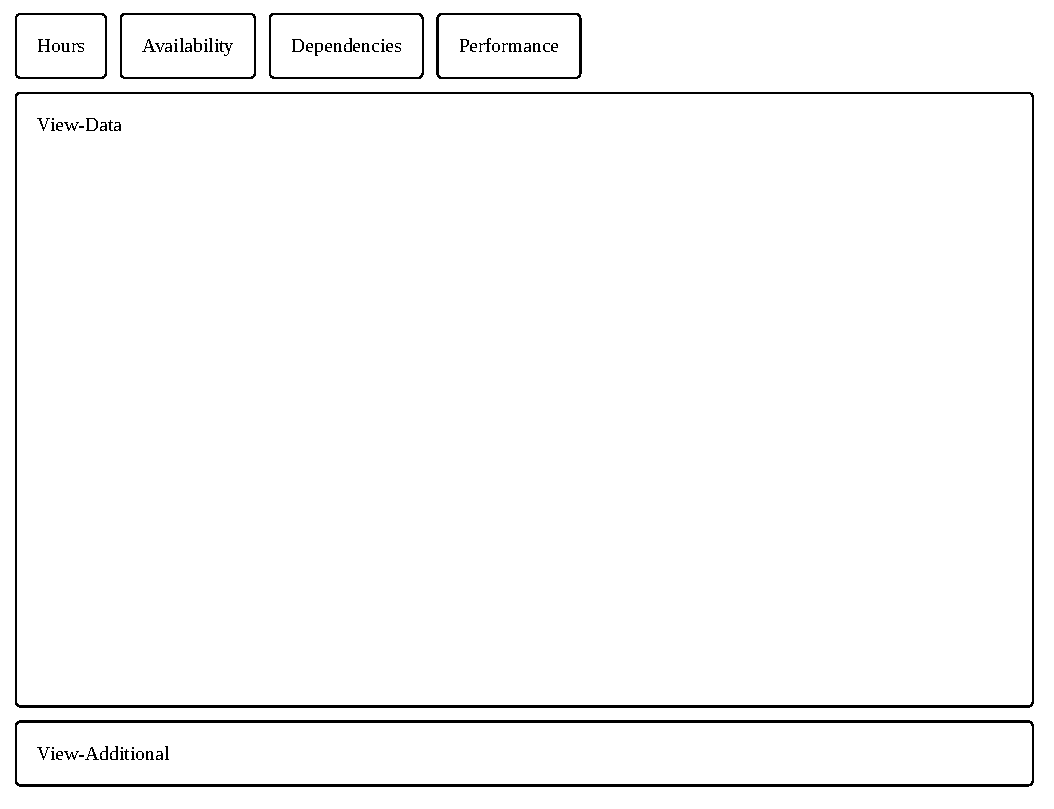
\includegraphics[width=\linewidth]{ui11.pdf}
          \end{minipage}
          \begin{minipage}{.49\textwidth}
            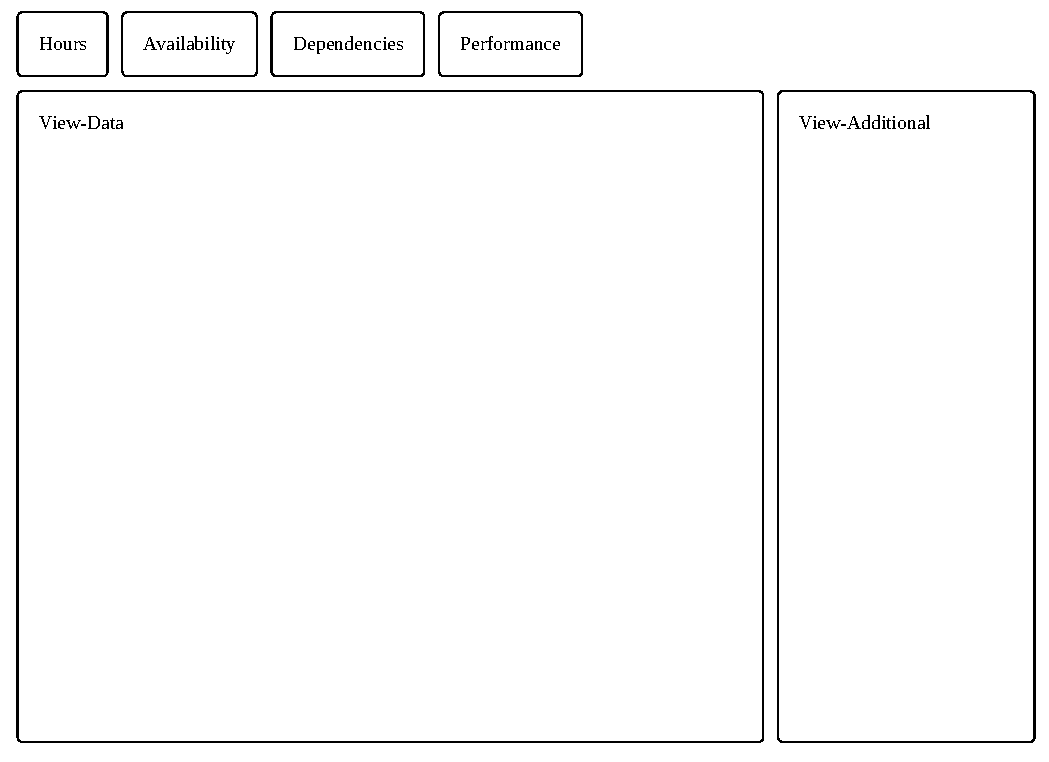
\includegraphics[width=\linewidth]{ui12.pdf}
          \end{minipage}
          \begin{minipage}{.49\textwidth}
            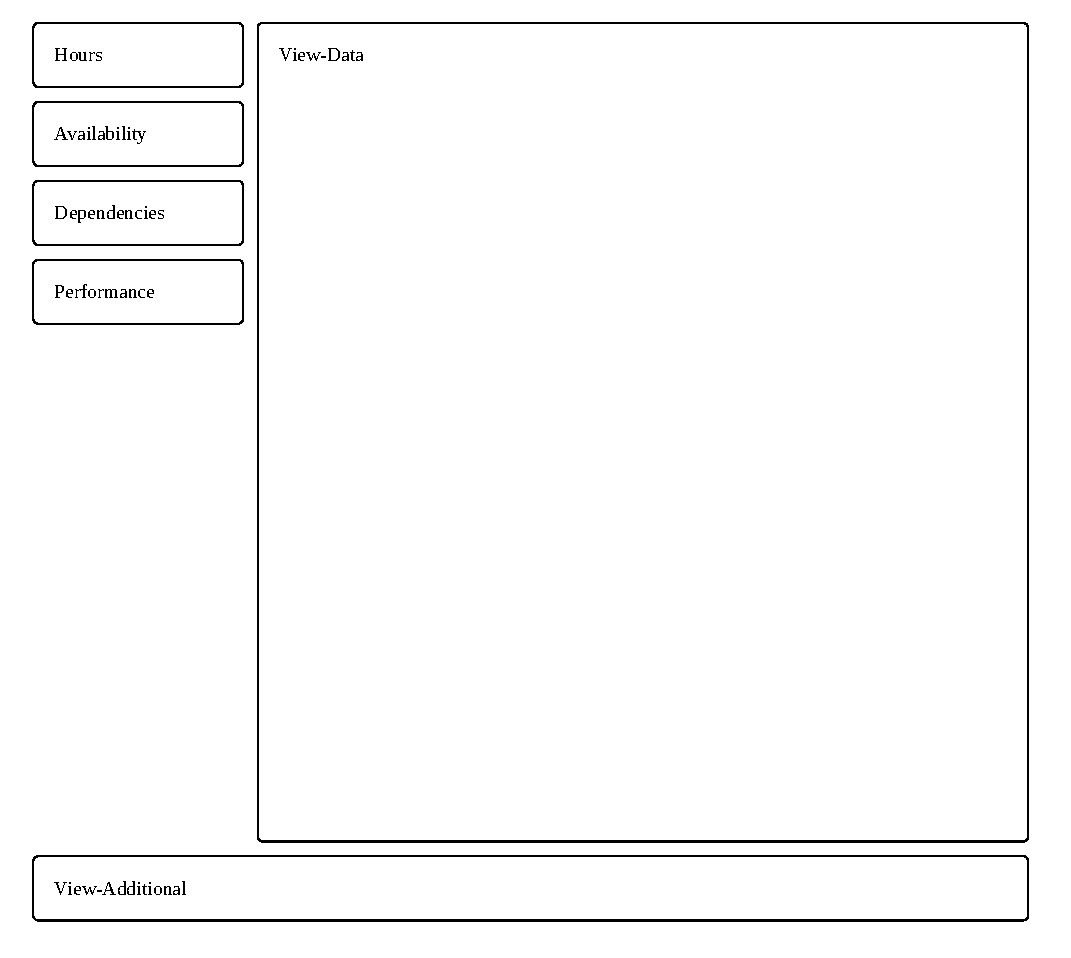
\includegraphics[width=\linewidth]{ui13.pdf}
          \end{minipage}
          \begin{minipage}{.49\textwidth}
            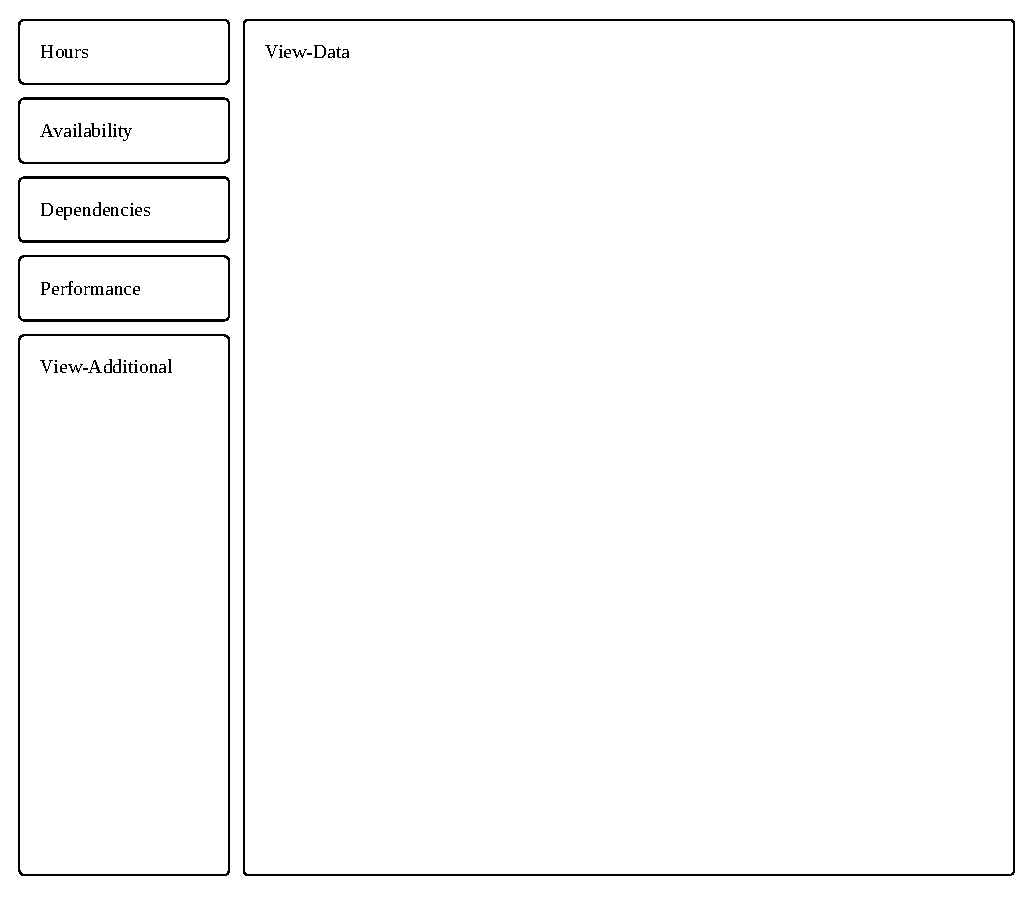
\includegraphics[width=\linewidth]{ui14.pdf}
          \end{minipage}
          \caption{Interface drafts 1.1, 1.2, 1.3 and 1.4.}
        \end{figure}

        \todoMaybe{These figures should probably be under result?}

        Four mock-up interfaces were created based on \todoInsert{part about
          ui design reference} and presented to five\checkTruth colleagues for
        evaluation. The evaluation was conducted as an in-person interview
        where the interviewee were asked to voiced their thoughts out aloud.
        After the initial reaction and thought about each of the designs, the
        interviewee was asked to pick, according to them, the most suitable
        design.

        After the initial pick, the interviewee was presented with
        \todoInsert{part about ISO-standard design}, which they had to arrange
        in order of most to least important according to their own views.
        After prioritizing the different design attributes, the participant was
        again asked to pick what they felt was the most suitable design.


        \todo{Expand with information about ISO design standard}

      \subsection{Gathering relevant test data}

        There is a two-fold goal that the collected test-data needs to solve:
        \begin{itemize}
          \item{
            Generate a quantifiable value that can be tracked in order to
            evaluate the participants performance during tests.
          }
          \item{
            Aggregate participant feedback about the platform in order to
            improve the next version.
          }
        \end{itemize}

        The first problem is solved by sticking with a established tradition
        within usability testing\findref\findref, measuring completion time.
        In order to keep track of their test-runs, participant are assigned an
        anonymous id-string after acknowledging that they have read the initial
        information. The anonymous id is registered as used in the database
        and the id is stored in the participants browsers web-session.

        As a participant starts a new task, the database will register the
        start-time and link it to the aforementioned anonymous id. If the
        participant completes the task, the stop-time will be recorded in the
        same database post, and the difference between these two values will be
        used as the time for task completion.

        Acquiring feedback data is done through a post-test survey with ten set
        questions (1-5) and a free-from dialog box for additional input.
        \todo{Expand and reword last section}


      \subsection{Evaluating impact and effectiveness}

        First the test-measurements and feedback is recorded from the
        participants and stored to the underlying database. This data can then
        be processed in order to find interesting correlations between
        different application variables, such as the test types impact on the
        overall completion time.

        The data is accumulated and processed using Python, specifically Python
        3.8.1 as of the time of this writing. The graphs included in this paper
        are generated through matplotlib, and numpy was used in select
        instances.

%        Since the data is stored in real-time and is available

%			Results by measuring the time and showing graphs + statistical grouping /
%			analysis.

		\section{Theory}

			\subsection{Information presentation and color}

        This looks into the interaction between the Human Visual System (HVS)
        and Graphical User Interfaces (GUIs), specifically the impact of color
        on this interaction.

        \todo{Expand section}

			\subsection{Representative high fidelity prototypes}

        User-Centered design and other iterative methods place a large
        importance on creating a high fidelity prototyp\findref that users can interact
        with, the sooner the better\findref.

        In order to create a high fidelity prototype from the paper prototypes
        presented earlier, each task had to be broken down into its essential
        component. All the given examples given from the managers revolved
        around identifying a specific piece of information, surrounded by
        similar data in order to act on it.

        \todo{Expand on 'finding a needle' approach with all the tasks, easy to
        time and evaluate.}


%			\subsection{Measuring time to task completion}
%
%
%        \todo{Expand section}

			\subsection{Thresholds for test failures}

        Is there a clear limit to when a participant should no longer be able
        to detect differences in color and relative sizes?

        \todo{Expand section}


		\section{Implementation}

      This section specifies how the user-facing web-application and its
      backend was constructed, and what the thought behind some of the
      decisions were.

%			Writing a web-application with Flask + python + sqlite3.
%			HTML5 and CSS with a dab javascript.

			\subsection{Platform software stack}

        The main user interfacing application is written in Python together
        with the Flask web-framework running on top of an Apache web-server.
        On the backend sqlite3 is used in order to store the results and
        feedback from participants for easy retrieval.

        While trying to keep the amount of JavaScript to a minimum, in order to
        have the highest possible interoperability rate, some snippets were
        required in order to make it possible to submit a web-form by clicking
        a SVG-graphic.

			\subsection{Interface creation}

        Interface wise the application is built in plain HTML5 markup to
        organize the main structure and buttons. All the various interfaces for
        the different tasks are constructed using Scalable Vector Graphics
        (SVG).

			\subsection{Variable challenges}

        Randomness provides a good source of test-material but is not a good
        fit for reproducibility. Fortunately this can be omitted by giving the
        random number generator a pre-determined seed as a parameter to its
        initialization call. Since the generator uses this seed as the basis
        for all the random number sequences it produces, in other words, the
        sequence of variables produced by two random number generators given
        the same seed should be identical.

        In this setup, the initial generator uses a hard-coded seed to to
        produce a few thousand unique alpha-numeric sequences that are then
        used as the anonymous ids for the participants. It is also these
        anonymous-ids that are used as the seeds when generating the different
        data-sets for each use.

        This makes it possibility to reconstruct a participants test by
        re-supplying the same anonymous-id and test-type to the application and
        it should return the same test-setup.


\addtocontents{toc}{\pagebreak}
	\chapter{Evaluation}

	  \chapter{Participants}

      Where from? \\

      How many? \\

      Section male / female / other. \\

      Average arg. \\

      Average test-session. \\


      \section{Participants where from?}

      \section{?}

    \section{Setup}

      \begin{itemize}
        \item{Upplägg på tester / vart gjordes de?}
      \end{itemize}

    \section{Procedure}

      \begin{itemize}
        \item{Informed Consent}
        \item{Number of tests}
        \item{question ares etc.}
        \item{picture of 'test-flow'}
      \end{itemize}

		\section{Results}

			\subsection{Pre-questionnaire -- itemizations}

        Before being able to perform the tests, each participant has to fill
        out and submit a pre-questionnaire. This is done in order to get
        a rough demographical overview of the people participating in this
        study. Initially they are asked about age, used input device, type of
        screen category the test were conducted on, and what binary gender, if
        any, they identify as.

				\begin{figure}[h!]
					\centering
					\includegraphics{figures/preQuestionnaireAnswers.pdf}
					\caption{Answers for the pre-questionnaire.}
				\end{figure}

        Beginning with age, with each dot representing one answer, no
        participant was twenty or below, most of the  participants were between
        twenty-one and thirty-five, with fourteen being thirty-six and older.
        Since a large part of the participants came from MASSIVE, this seems to
        fit the mean age at the company, which is at thirty-two{\findref} at
        the time of this writing.

        It's is worth mentioning however, that the most represented single age
        was twenty-five, which is the default value set for the age input
        field. More on this specifically in \todoInsert{Link to threats to
          validity}.

				\begin{figure}[h!]
					\centering
					\includegraphics{figures/preQuestionnaireAnswersIdentify.pdf}
					\caption{Answers for the pre-questionnaire.}
				\end{figure}

        Asking people for what gender they identify as results in the largest
        group, 52 participants, identify as male. Again, as a large portion of
        participants came from MASSIVE, this is expected since the gender
        distribution in businesses related game-development tend to be weighted
        toward men\findref\findref.

				\begin{figure}[h!]
					\centering
					\includegraphics{figures/preQuestionnaireAnswersInputs.pdf}
					\caption{Answers for the pre-questionnaire.}
				\end{figure}

        Continuing the trend, most workstations at MASSIVE consist of a
        desktop PC where the main peripherals used for input are a mouse and a
        keyboard with the occasional drawing tablet mixed in.

        In general it was assumed that most of the participants were going to
        use a mouse and keyboard, with trackpads as a probable second place,
        making the turnout of nearly twenty participants using touch as their
        main input a bit of a surprise.

        Even though the assumed main input method for these tests is a keyboard
        and mouse at a stationary desktop computer, the overarching goal of the
        project, as stated earlier, is to be a pre-cursor to o more generalized
        usability testing framework. In order to align with this goal, it is
        important to explore the possibility of scaling the interface and
        related tests to different screen sizes, and analyze what, if any,
        impact is has on participant performance.

				\begin{figure}[h!]
					\centering
					\includegraphics{figures/preQuestionnaireAnswersScreen.pdf}
					\caption{Answers for the pre-questionnaire.}
				\end{figure}

        Requiring actual screen-sizes was seen as to cumbersome of a task to
        ask of the participants, especially if using devices other than a
        somewhat standard desktop monitor. Here the categories roughly equate
        to; \textit{Desktop}: 18" or larger, \textit{Laptop}: 13"-17", \textit{Tablet}:
        11"-12" and \textit{Mobile}: 10" and below.

			\subsection{Pre-questionnaire -- 1-5 questions}

        Aside from the physical setup, there are relevant knowledges and
        experience that could become interesting when analyzing free-form
        answers and test-results gathered from the participants. As an example,
        is the free-form feedback different from someone that is interested in
        usability-design? Does the level of computer literacy or experience
        with mouse-driven games impact completion times? Etcetera.

        In order to evaluate these aspects the second half of the
        pre-questionnaire included five self-evaluation-1-to-5 questions
        \todo{Find the actual name}, questions and answer distribution
        displayed below:

				\begin{figure}[h!]
          \textbf{Q1: I feel comfortable using a computer.}
          \begin{center}
            \includegraphics[width=\linewidth]{figures/preQuestionnaireAnswersOneToFive.pdf}
            \vspace{-1cm}
            \caption{Answers for the pre-questionnaire Q1.}
          \end{center}
				\end{figure}

        The clear majority of participants feel that they are very comfortable
        using a computer. Since this question is so heavily skewed towards
        \textit{Strongly agree}, it would be interesting to add an additional
        \textit{I see myself as an advanced computer user} or similar in order
        to try to separate out more divisions.

				\begin{figure}[h!]
          \textbf{Q2: I have a interest in UI-design.}
          \begin{center}
            \includegraphics[width=\linewidth]{figures/preQuestionnaireAnswersOneToFiveQ2.pdf}
            \vspace{-1cm}
            \caption{Answers for the pre-questionnaire Q2.}
          \end{center}
				\end{figure}

        Looking at the general interest in regards to user interface design,
        most participants either do not care about it, or find it somewhat to
        very interesting. If this was a non-anonymous study, it would be
        interesting to follow up on the seven participants that strongly
        disagree to this question. Mostly in order to differentiate if they do
        not like user interfaces an input method in general, or if it is more
        related to them not wanting to be involved in user interface design.

				\begin{figure}[h!]
          \textbf{Q3: I have studied UI-design.}
          \begin{center}
            \includegraphics[width=\linewidth]{figures/preQuestionnaireAnswersOneToFiveQ3.pdf}
            \vspace{-1cm}
            \caption{Answers for the pre-questionnaire Q3.}
          \end{center}
				\end{figure}

        In terms of having studied user interface design, the majority of
        participants have not. Since this is a pure self-assessment, the
        definition of what \textit{studied} means in this context is up for
        grabs. A follow up question in regards to what type of study;
        self-learnt, online-course, university etcetera would be needed clarify
        this information further.

				\begin{figure}[h!]
          \textbf{Q4: I play pointer based games (e.g. first person shooters).}
          \begin{center}
            \includegraphics[width=\linewidth]{figures/preQuestionnaireAnswersOneToFiveQ4.pdf}
            \vspace{-1cm}
            \caption{Answers for the pre-questionnaire Q4.}
          \end{center}
				\end{figure}

        A slight majority agree, in some capacity, that they play games where
        the main form of input is pointer movements. Following this question
        with one that seeks to answer the underlying reason why disagreeing
        participants do not interact more with this kind of games could be
        interesting from a interface design standpoint. Additional questions or
        follow-up would be needed to determine if the disagreement it is a
        matter of taste, design faults, available time, or something completely
        different.

				\begin{figure}[h!]
          \textbf{Q5: I have trouble distinguishing some colors from each other.}
          \begin{center}
            \includegraphics[width=\linewidth]{figures/preQuestionnaireAnswersOneToFiveQ5.pdf}
            \vspace{-1cm}
            \caption{Answers for the pre-questionnaire Q5.}
            \vspace{-0.4cm}
          \end{center}
				\end{figure}

        All of the available tests incorporates different color pallets to
        varying degree, which makes it interesting to know if any of the
        participants have trouble making out the difference between colors.
        \vspace{-0.6cm}

			\subsection{Launch, participation and overall success ratio}

        The test-site went live 2020-01-24 with the link initially shared only
        through Facebook. On 2020-01-27 the link was shared on the MASSIVE
        internal mailing list, boosting the participation significantly.
        In total, \varHere{totalParticipants} participants moved past the
        initial information over a five day period.

        \vspace{-0.55cm}
				\begin{figure}[h!]
					\centering
					\includegraphics{figures/participantsOverTime.pdf}
          \vspace{-0.3cm}
          \caption{
            Total amount of participants that got past the initial
            information screen and did not abort the tests.
          }
				\end{figure}

				In total \varHere{totalTests} tests were run, where
				\varHere{totalTestsCorrect} were answered correctly,
				\varHere{totalTestsUncompleted} never produced an answer, leaving
				\varHere{totalTestsIncorrect} incorrect answers. Looking only on the test
				runs without any user- or task-correlation, the chance that any given test run
				produces the correct answer is $\sim$\varHere{varTotalRatioSuccess}\%.

				\begin{figure}[h!]
					\centering
					\includegraphics[width=0.95\linewidth]{figures/runsOverTime.pdf}
          \vspace{-0.3cm}
          \caption{Lines representing total amount of test-runs together with
            the total of runs that produces the correct answer.}
          \vspace{-0.4cm}
				\end{figure}

			\subsection{Tests per user and defining outliers}

				The number of recommended test was five, which when completed, allowed
				the participant to continue to the final survey. However, there was
				nothing stopping each participant from doing more or less than five.
        By generating a histogram for the number of performed tests per
        participant it is possible to determine which of tests was most
        popular.

				\begin{figure}[h!]
					\centering
					\includegraphics{figures/testsPerUser.pdf}
					\caption{Participants grouped on how many test they performed.}
				\end{figure}

        In total, of the \varHere{totalParticipants} number of participant that
        started a session, \varHere{valNumAnyTestsRun} of them ran at least one
        test, which means \varHere{valTestNoTests} ran no tests. Retrieving and
        tabulating additional values, discarding users with no test-runs,
        produces the following table.
        %Further more, \varHere{valTestsFiveToTen} completed between
        %five and nine tests, and \varHere{valTestsElevenOrMore} completed ten or
        %more. (\varHere{valTestTenOrLessP}) (\varHere{valTestsElevenOrMoreP})

        \begin{figure}[h!]
          \centering
          \varHere{tablePrecentageOfUsers}
          \caption{
            Tabulated values of test-run groups with corresponding percentage
            of total active participants.
          }
        \end{figure}

        Participants that have run at most fifteen tests make up slightly more
        than 91\% of the total number of participants and will be the regular
        group, denoted as $\#r\leq15$. Inversely the remaining participants
        that have run sixteen or more tests in total, $\sim$9\% of the total
        amount of participant will be seen as the outlier group, denoted as
        $\#r\geq16$.

      \subsection{Test type distribution among participants}

        There are no restrictions in place in regards to how a participant
        can choose which task types to preform in what order. By grouping all
        the task-runs based on the type of the task, it is possible to see if
        any type is more popular than the others.

				\begin{figure}[h!]
					\centering
					\includegraphics{figures/testsRunPerTask.pdf}
          \caption{
            Distribution of task types among all total runs together with the
            total for the regular- and outlier-grouping respectively.
          }
				\end{figure}

        Examining the types distributed over all participants together
        with the different groupings, \textit{Employee Hours} is the most
        executed test type, regardless of categorization.

				\begin{figure}[h!]
					\centering
					\includegraphics{figures/testsRunPerTaskOutliers.pdf}
          \caption{
            Detailed breakdown of task distribution for the outliers, multiples
            of identical distributions removed.
          }
          \label{label_testsRunPerTaskOutliers}
				\end{figure}

        Taking a closer look at the distribution in the outlier group,
        $\#r\geq16$, reveals that almost all of them, six out of the total seven,
        are symmetrically split between all four task-types. Out of the sums
        [20, 20, 20, 32, 49, 100], it is only 49 that is not evenly divisible
        by four. This has the added effect that the participants in the
        outlier grouping, even though they might have ran the most total tests
        comparatively, do not impact the type distribution since a symmetrical
        distribution cancels itself out in this case.

      \subsection{Checking for preferential task order}

        As with the task-types, there are no no restrictions on in what order a
        participant can preform tasks. Grouping the tasks for each participant
        and sorting them in chronological order results in a view into what
        order each participant choose to run the different tasks.

				\begin{figure}[ht!]
					\centering
					\includegraphics{figures/testsRunOrder.pdf}
          \caption{
            Bar-graph showing the ratio of specific task-types depending on the
            the chronological order of the run.
          }
          \label{label_testsRunOrder}
        \end{figure}

        Since the legend in figure \ref{label_testsRunOrder} reflects the order
        in which the tasks appear in the user interface for participants, the
        majority choose to do the tasks in the presented order, top to bottom.
        As for the fifth test run, the majority choose do an extra of the last
        one (Team Performance), and after that, most participants opted to go
        back and do the first one again (Employee Hours).

        Given the wider range of the data coming from the outlier group (1-100)
        the visualization needs to be altered slightly. Since there is not
        enough room to have the bars side by side, they have been stacked, with
        the largest bar being at the bottom.
				\begin{figure}[ht!]
					\centering
					\includegraphics{figures/testsRunOrderOutliers.pdf}
          \caption{
            Stacked bars showing relation between task order and task type for
            the outlier group.
          }
				\end{figure}

        Initially the going-by-order tendency from figure
        \ref{label_testsRunOrder} holds for index one and two, but breaks down
        on the third, with the second option being the most prevalent.
        Interestingly, the sequential does appears between run five and nine,
        then disappears. Apart from that, it seems the preferable way to do
        thirty or more tests is to do them in batches.

        Exact values this figure and number of users in each group can be found
        tabulated in the appendix. \todo{Add table and reference}

%      \todo{
%        Continue exploring the data, time distribution? Which task was failed
%        the most? Are there thresholds in the variables where tasks start to
%        fail more often? Is there a most preferable order to do the tasks?
%        Which task is the most popular in the 5-run category? ...
%      }
%

      \subsection{Success-rates and task type}

        When completing a test-run the application marks the result as
        either correct or wrong in the underlying database. Extracting
        those answers and grouping them by the task-type makes it possible to
        compare the relative success- and failure-rates for each task-type.

				\begin{figure}[h!]
					\centering
          \includegraphics{figures/testsResultsByType.pdf}
          \caption{
            Bars showing percentages of all answers that are correct for a
            given task-type for regular and outlier groupings.
          }
				\end{figure}

        Reading the graph, the difficulty of the task-types in order of hardest
        to easiest is as follows: \textit{Employee Hours} is the hardest to get
        correct, followed by \textit{Team Performance}, \textit{Team Workload}
        and finally, the easiest to get a correct answer on, \textit{Task
          Dependencies}. According to the same data, the outlier group seems to
        be on average, more correct than the regular group.

%        Given that the data seems to suggest that success-rate increases with
%        the number of performed tasks, the data is re-arranged to show the
%        percentage of correct answer mapped against the task run index, shown
%        below:

%				\begin{figure}[ht!]
%					\centering
%          \includegraphics{figures/testsResultsByTaskIndex.pdf}
%          \caption{
%            Percentages of correct task answers split on ordinary and outlier
%            groups.
%          }
%				\end{figure}

%				\begin{figure}[ht!]
%					\centering
%          \includegraphics{figures/testsResultsByTaskIndexAndTestType.pdf}
%          \caption{
%            Percentages of correct task answers split on ordinary and outlier
%            groups.
%          }
%				\end{figure}
%
      \subsection{Completion times - Task types and distribution}

        Computing the mean and average completion time for the task-runs is
        simply a matter of gathering all the start and stop times from the
        database and perform the corresponding arithmetics. The resulting times,
        split in regular and outliers, is shown below.

        \begin{figure}[h!]
          \centering
          \includegraphics{figures/testsTimesPerTaskTypeOutliers.pdf}
          \vspace{-0.3cm}
          \caption{Average and median completion times for task-types. }
          \label{label_testsTimesPerTaskTypeOutliers}
        \end{figure}


        \textit{Employee Hours} has, according to the data, the longest average
        and median completion time of all the task types, which holds for both
        groupings. This makes sense since that the earlier analysis, looking at
        the overall success-rate for different tasks-types, points to
        \textit{Employee Hours} being the hardest task type of the four.

        By adding a few percentiles to a histogram based on the completion times for all
        tasks and participants, it is possible to determine that that 50\% of
        all tasks-runs were completed in 7 seconds or less, 90\% in 10 seconds
        or less and 95\% of all runs completed below 42 seconds.

        \begin{figure}[h!]
          \centering
          \includegraphics{figures/testsTimeGroupingsTotal.pdf}
          \caption{
            Histograms showing groupings of completion-times for all users
            rounded to nearest second.
          }
        \end{figure}

        Reusing the previous data by splitting it and creating one histogram
        each for the regular and outlier group gives a better view of how the
        completion times are distributed for each of the groups respectably,
        result shown below.

        \begin{figure}[h!]
          \centering
          \includegraphics{figures/testsTimeGroupings.pdf}
          \caption{
            Histograms showing groupings of completion-times rounded to nearest
            second for; all, regular and outliers user-groups.
          }
        \end{figure}

        For the outlier group, 50\% of all tests were completed in 3 seconds or
        less, compared to 9 seconds or less for participants in the regular
        group. This pattern is repeated for the 90th percentile, where 90\% of
        the tests in the outlier group were completed in 9 seconds or less,
        compared to 35 seconds or less in the regular group.

			\subsection{Effect of color pallet on completion times}

        \todo{Figure out a good way to calculate and visualize this.}

			\subsection{Largest impact on completion times}

        \todo{Possible multi variat analysis? Possible? Worth it?}

			\subsection{Post-survey questions}

        In order to gather feedback for evaluation and possible incorporation
        into the next design iterations, the test concludes with a second
        questionnaire with eight '1-5 questions'. These questions are ment to
        evaluate what participants thought about the setup, and if they have
        any suggestions, comments or improvements.

				\begin{figure}[h!]
          \textbf{Q1: The goal of each task was clear.}
          \begin{center}
            \includegraphics[width=\linewidth]{figures/postQuestionnaireAnswersOneToFiveQ1.pdf}
            \vspace{-1cm}
            \caption{Answers for the post-questionnaire Q1.}
          \end{center}
				\end{figure}

        One of the main goals was to only challenge the participants in the
        time it took them to complete a task and make it as easy for them every
        where else. This means that there should be as little confusion to what
        needs to be done in order to satisfy a test, and the challenge should
        come from selecting one of many well understood options. And since a
        clear majority at least agree that each task goal was clear, this goal
        was accomplished.

				\begin{figure}[h!]
          \textbf{Q2: Test-application looks good.}
          \begin{center}
            \includegraphics[width=\linewidth]{figures/postQuestionnaireAnswersOneToFiveQ2.pdf}
            \vspace{-1cm}
            \caption{Answers for the post-questionnaire Q2.}
          \end{center}
				\end{figure}

        While appreciating that the majority of participants was either
        indifferent or liked the design of the application, it was not one of
        the goals for this project. The main goal was to be usable and scaling
        well to different media sizes, not looking good.

        This reads either as the participants being nice since the tone of the
        project is personal, or the design was too polished. If the latter case
        is true, it indicates that this first iteration should have been in the
        hands of participants sooner.

				\begin{figure}[h!]
          \textbf{Q3: Use of colors helped with the tasks.}
          \begin{center}
            \includegraphics[width=\linewidth]{figures/postQuestionnaireAnswersOneToFiveQ3.pdf}
            \vspace{-1cm}
            \caption{Answers for the post-questionnaire Q3.}
          \end{center}
				\end{figure}

        Most people agreed that the color helped them preform their tasks.
        This question could be augmented with additional questions that asks
        more specifically about the perceived help. Additionally, it could be
        complemented with a permutation of runs that do not contain any color,
        in order to gather some test-data about runs without color.

				\begin{figure}[h!]
          \textbf{Q4: Amount of information was adequate.}
          \begin{center}
            \includegraphics[width=\linewidth]{figures/postQuestionnaireAnswersOneToFiveQ4.pdf}
            \vspace{-1cm}
            \caption{Answers for the post-questionnaire Q4.}
          \end{center}
				\end{figure}

        The Majority answered that the information that they were provided was
        adequate. Again, it would be very interesting to ask the participants
        that disagree what they felt was missing.

				\begin{figure}[h!]
          \textbf{Q5: Test-application is easy to to navigate.}
          \begin{center}
            \includegraphics[width=\linewidth]{figures/postQuestionnaireAnswersOneToFiveQ5.pdf}
            \vspace{-1cm}
            \caption{Answers for the post-questionnaire Q5.}
          \end{center}
				\end{figure}

        As stated earlier, participants should only need to apply them self
        when doing the actual tests. The goal is that the navigation should be
        easily traversable, which the majority of participants seem to agreed with.

				\begin{figure}[h!]
          \begin{center}
            \textbf{Q6: Appropriate choice of colors.}
            \includegraphics[width=\linewidth]{figures/postQuestionnaireAnswersOneToFiveQ6.pdf}
            \vspace{-1cm}
            \caption{Answers for the post-questionnaire Q6.}
          \end{center}
				\end{figure}

        The questionnaire shows that most participant thought that choice of
        colors were appropriate.

				\begin{figure}[h!]
          \textbf{Q7: Language used was easy to understand.}
          \begin{center}
            \includegraphics[width=\linewidth]{figures/postQuestionnaireAnswersOneToFiveQ7.pdf}
            \vspace{-1cm}
            \caption{Answers for the post-questionnaire Q7.}
          \end{center}
				\end{figure}

        A majority of participants agreed that the language used in the
        application was easy to understand, with none of the participants
        strongly disagreeing with the statement.

				\begin{figure}[h!]
          \textbf{Q8: Easy to understand what to do next.}
          \begin{center}
            \includegraphics[width=\linewidth]{figures/postQuestionnaireAnswersOneToFiveQ8.pdf}
            \vspace{-1cm}
            \caption{Answers for the post-questionnaire Q8.}
          \end{center}
				\end{figure}

        It is encouraging that most participants felt that they knew what to do
        next when performing the tests. It would of course be preferable if
        every one felt they knew what to do, but the result is encouraging.

		\section{Discussion}

      \subsection{The development process}


        \begin{itemize}
          \item{Discuss the process. Good bad? Done anything differently?}
          \item{}
          \item{}
          \item{}
        \end{itemize}

      \subsection{Results}

        \begin{itemize}
          \item{Discuss the results.}
          \item{Anything weird?}
          \item{Everything as planned?}
          \item{Outliers, why?}
        \end{itemize}

			\subsection{Possible improvements}

        What could be improved if this was done again?

        \subsubsection{Multiple design iterations}

          Should have had multiple smaller iterations, easy to get stuck.

        \subsubsection{Opt-in followup}

          Some questions reveled answers that didn't match what I had
          anticipated, would be interesting to at least have a chance to follow
          up on those observations.

        \subsubsection{Leverage more frameworks?}

          Didn't have the foundational expertise to deicide on a good
          framework, would be easier now.
          Build upon frameworks for faster iteration?

			\subsection{Threats to validity}

        \subsubsection{Online testing and latency}

          Latency should be minimal, but it would be better to measure and
          verify than simply guess.

        \subsubsection{Seeding with user-id}

          Might be a quirk in that re-seeding with the same user-id could
          possibly create 'easy' anonymous id's.



%				network latency?
%				multiple runs with same person?



	\chapter{Conclusions}

		Did it have an significant impact? Was the web the correct platform? What
		could be done better over the internet? Recording screen and voice?
		(Javascript, since it's already used, pull up some statistics?)

	% Should use consistent formatting when it comes to Names ("FirstName LastName", or "F. LastName")
	\makebibliography{report}

	%make sure we're on even page with the pop-sci
	\checkoddpage
	\ifoddpage
	\else
		 \newpage
		 \thispagestyle{empty}
		 \mbox{ }
	\fi
	%\begin{appendices}
	%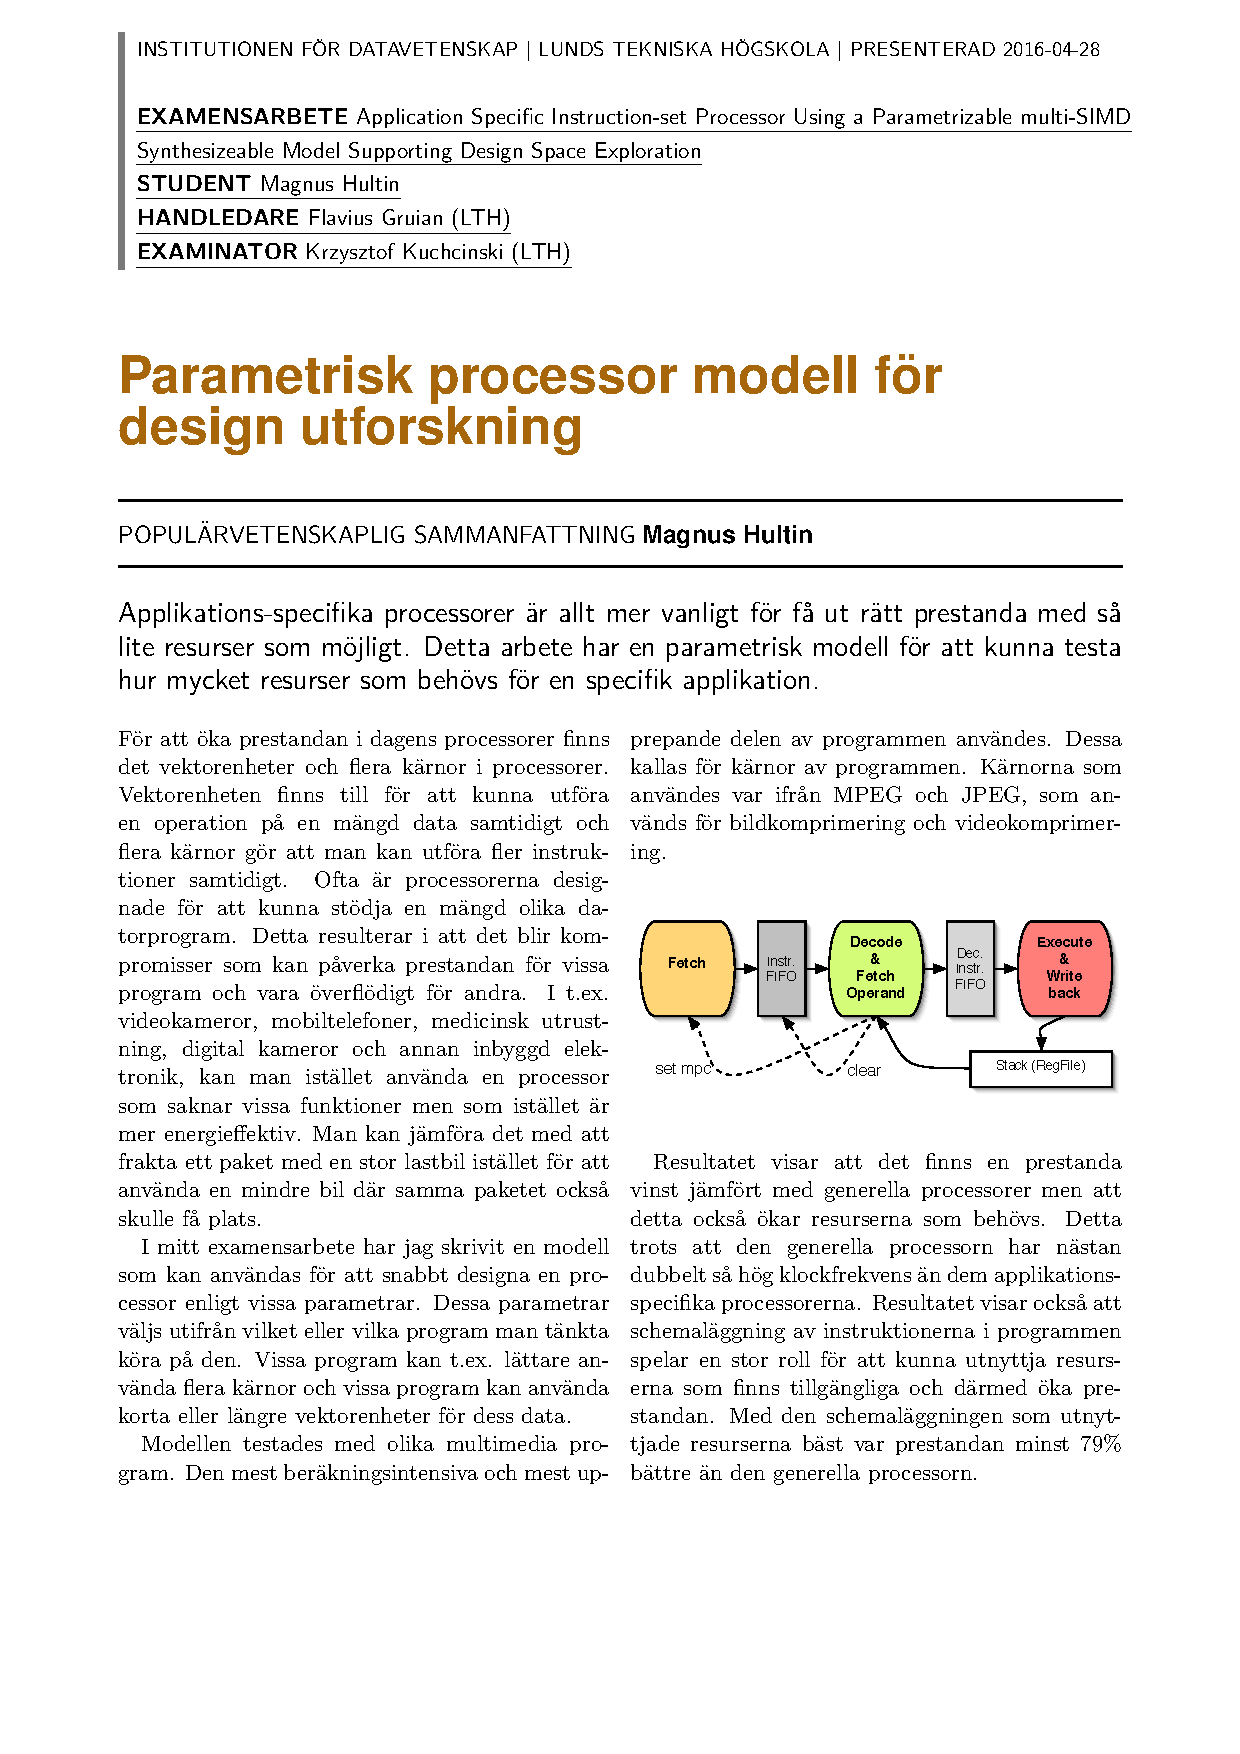
\includepdf[pages={1}]{popsci/popsci.pdf}
	%\end{appendices}

  \chapter{Appendix}


        \begin{figure}[h!]
          \centering
          \includegraphics{figures/testsTimeGroupingsHours.pdf}
          \caption{
            Histograms showing groupings of completion-times rounded to nearest
            second for; all, regular and outliers user-groups.
          }
        \end{figure}

        \begin{figure}[h!]
          \centering
          \includegraphics{figures/testsTimeGroupingsWorkload.pdf}
          \caption{
            Histograms showing groupings of completion-times rounded to nearest
            second for; all, regular and outliers user-groups.
          }
        \end{figure}

        \begin{figure}[h!]
          \centering
          \includegraphics{figures/testsTimeGroupingsDependencies.pdf}
          \caption{
            Histograms showing groupings of completion-times rounded to nearest
            second for; all, regular and outliers user-groups.
          }
        \end{figure}

        \begin{figure}[h!]
          \centering
          \includegraphics{figures/testsTimeGroupingsPerformance.pdf}
          \caption{
            Histograms showing groupings of completion-times rounded to nearest
            second for; all, regular and outliers user-groups.
          }
        \end{figure}

\end{document}
